\scanpage{73}
\margin{- 139 -}
\margin{IX}

définir l'isomorphisme canonique (11.6.2).

Ecrivant $M_\ell\otimes D_\ell$ (resp. $\check M_\ell\otimes D_\ell$) comme limite inductive des $M_n$ (resp. des $\check M'_n$), où $n$ parcourt les puissances de $\ell$, il revient au même de définir (11.6.2), où des isomorphismes canoniques
\[
(11.6.4)\qquad {}_n\Phi_o\simeq\operatorname{Ker}
\{\widetilde u_n:M_n\longrightarrow\check M'_n),\quad n=\ell^{r+1},
\]
comptatibles avec les morphismes de transition évidents, pour $n$ variable
(où $\widetilde u_n$ désigne maintenant, par abus de notations, l'homomorphisme déduit de $\widetilde u_\ell:M_\ell\longrightarrow\check M'_\ell$ par réduction mod. $n$).

Pour ceci, considérons le schéma en groupes $ {}_n A$ sur $S$, qui est plat et quasi-fini sur $S$ (2.2.1), grâce à l'hypothèse de réduction semi-stable. On a une filtration canonique
\[
(11.6.5)\qquad {}_n A\supset({}_n A^o)^f\supset({}_n A^o)^t\supset0,
\]
où l'exposant $f$ (resp. l'exposant $t$) désigne la ``partie fixe'' (2.2.3) (resp. la ``partie torique'' (5.1)) du schéma en groupe qu'il affecte ; pour la définition de la partie torique dans 5.1, on notera qu'on avait supposé $S$ complet, ce qui est loisible ici (11.0). (On a d'ailleurs vu dans 6.1 que la construction se généralise au cas $S$ hensélien, si on y tient \ldots) Soit
\[
(11.6.6)\qquad {}_n\Psi={}_n A/({}_n A^o)^f,
\]
c'est un schéma en groupes plat, séparé et quasi-fini sur $S$ (SGA 3 $\mathrm{VI}_A$ 3.2 et $\mathrm{VI}_B$ 9.2) de fibre générique
\[
{}_n\Psi_K=({}_n A_K)/({}_n A_K)^f,
\]

\margin{\figure{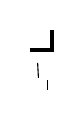
\begin{tikzpicture}
\draw[line width=1.5pt] (0,.4)--(.28,.4)--(.28,.66);
\draw (.1,.24)--(.11,.05);\draw (.22,.02)--(.22,-.1);
\end{tikzpicture}}}
\margin{\unsure{457}}
\margin{\unsure{13|B}}
\margin{457}
\margin{72}
